This chapter includes the introduction to the topic to be studied during this Bachelor's Thesis along with the reasoning behind choosing it and its structure. Information regarding the socio-economic environment and regulations that apply are also included here.

\section{Background}
Information has usually been referred to as one of the key aspects that every learning system needs in order to increase its capabilities and improve its performance. This is especially relevant for the Data Analytics field and the process of designing machine learning applications, where many experts usually refer to information as a powerful metric to indicate the success of their architecture at solving a particular problem. Due to the plethora of works already available online to master and use different techniques, the goal of this work is to asses the capabilities of these techniques and discuss its informational properties. 

%\setlength{\parindent}{10ex}

During the last few years, the topic of Big Data has become increasingly more important in our society. It is currently being used or developed in almost every industry in the world~\cite{article_Big_Data} and it is growing faster every day. While methods like Deep Neural Networks are beginning to be  widely available,  researchers tend to use the same approaches and steps to get their results. Rather than trying new methods, it is an industry standard to use a certain set of techniques when presented with a type of problem and then to try to optimize them. It is just assumed that these methods are powerful enough to find a suitable answer. 

A conceptual diagram of this model can be found in Figure~\ref{fig:fig1}.\subref{fig:fig1b}, where each block represents a different function inside an end-to-end informational model. Suppose we could only take measures outside each of the blocks and the contents or the methods being used inside are outside of the scope of the task. By not being able to access each one of the blocks to evaluate the processes inside them, we may only fix or change their inputs to try to improve our results.
%
\begin{figure}[H]
	\begin{subfigure}{1\textwidth}  
		\centering
		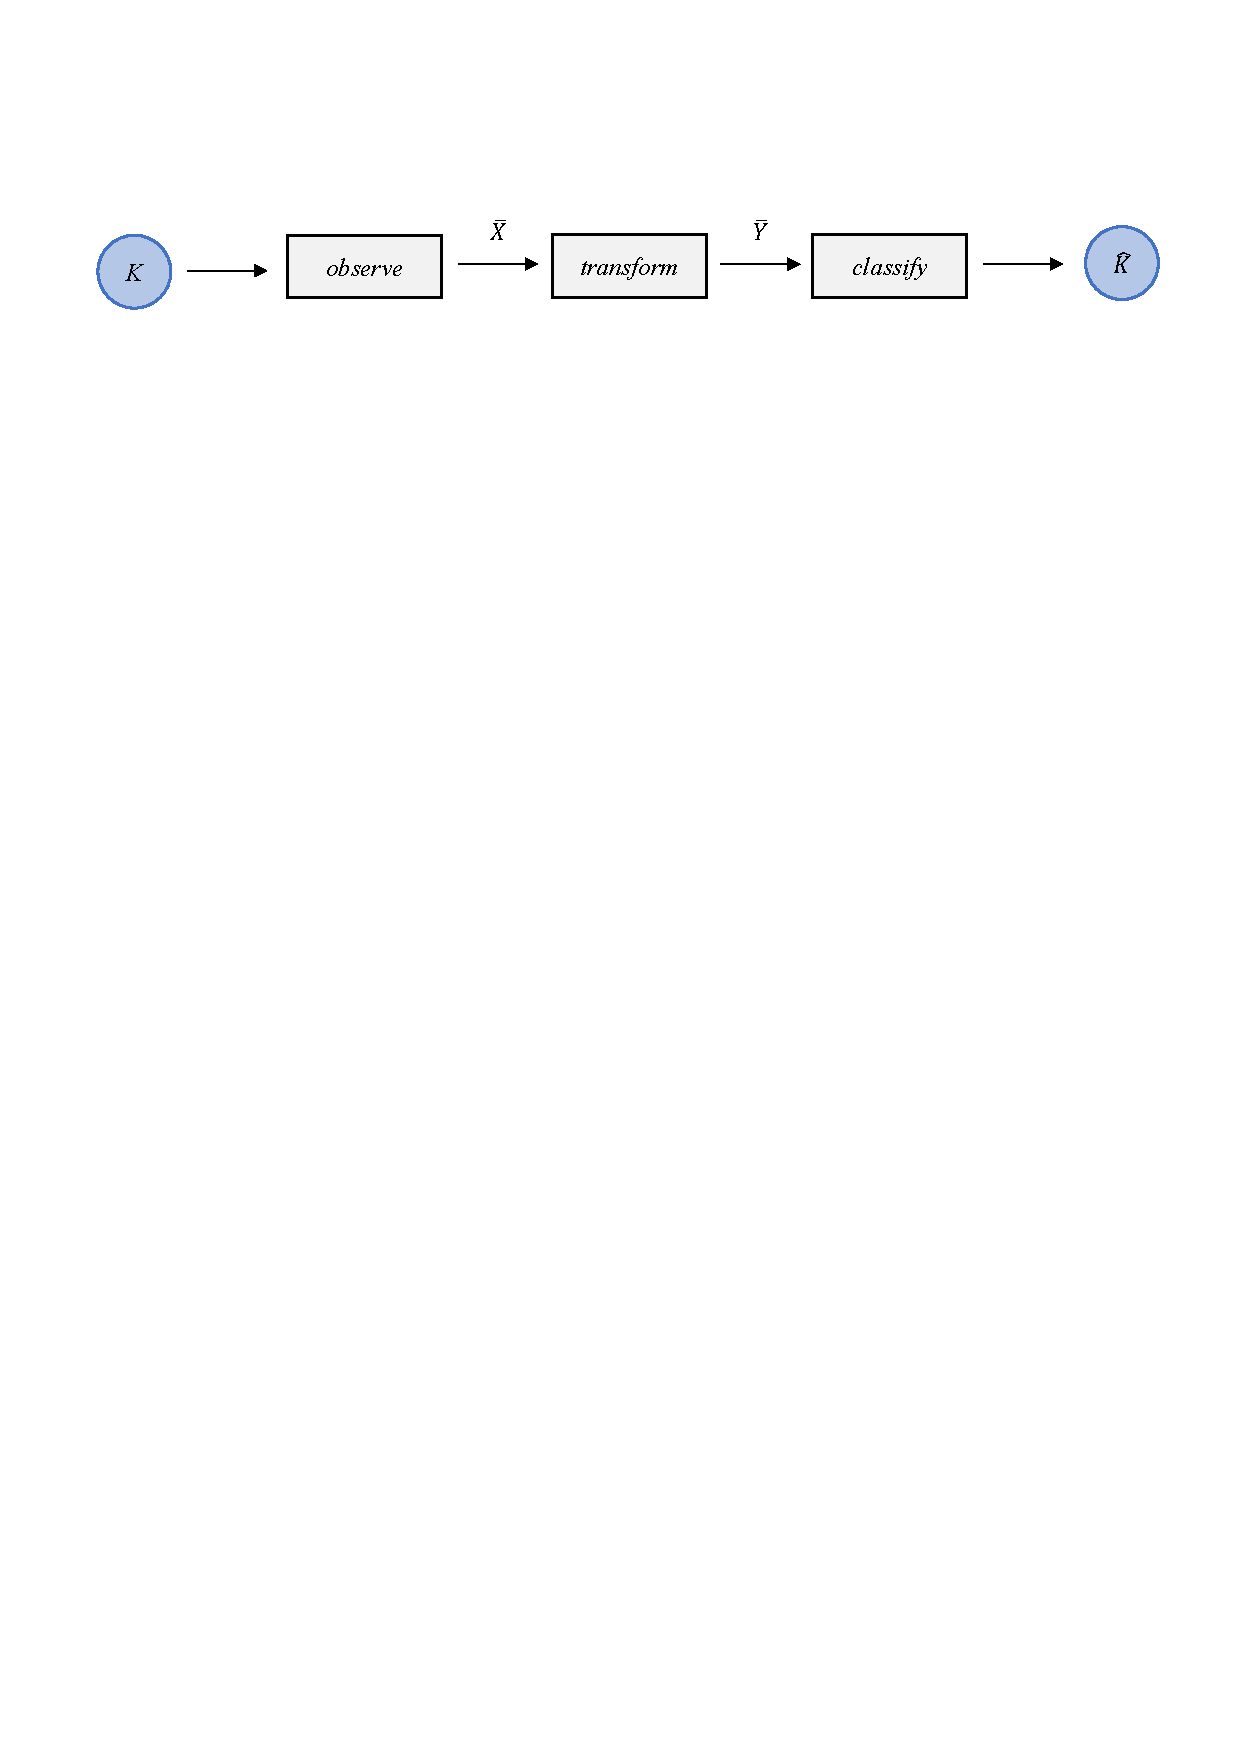
\includegraphics[width=16cm]{Figuras_tfg/Figura1_tfg}
		\caption{Conceptual representation of a classification process as a communication scheme.}
		\label{fig:fig1b} 
	\end{subfigure}%  
	
	\begin{subfigure}{1\textwidth} 
		\centering
		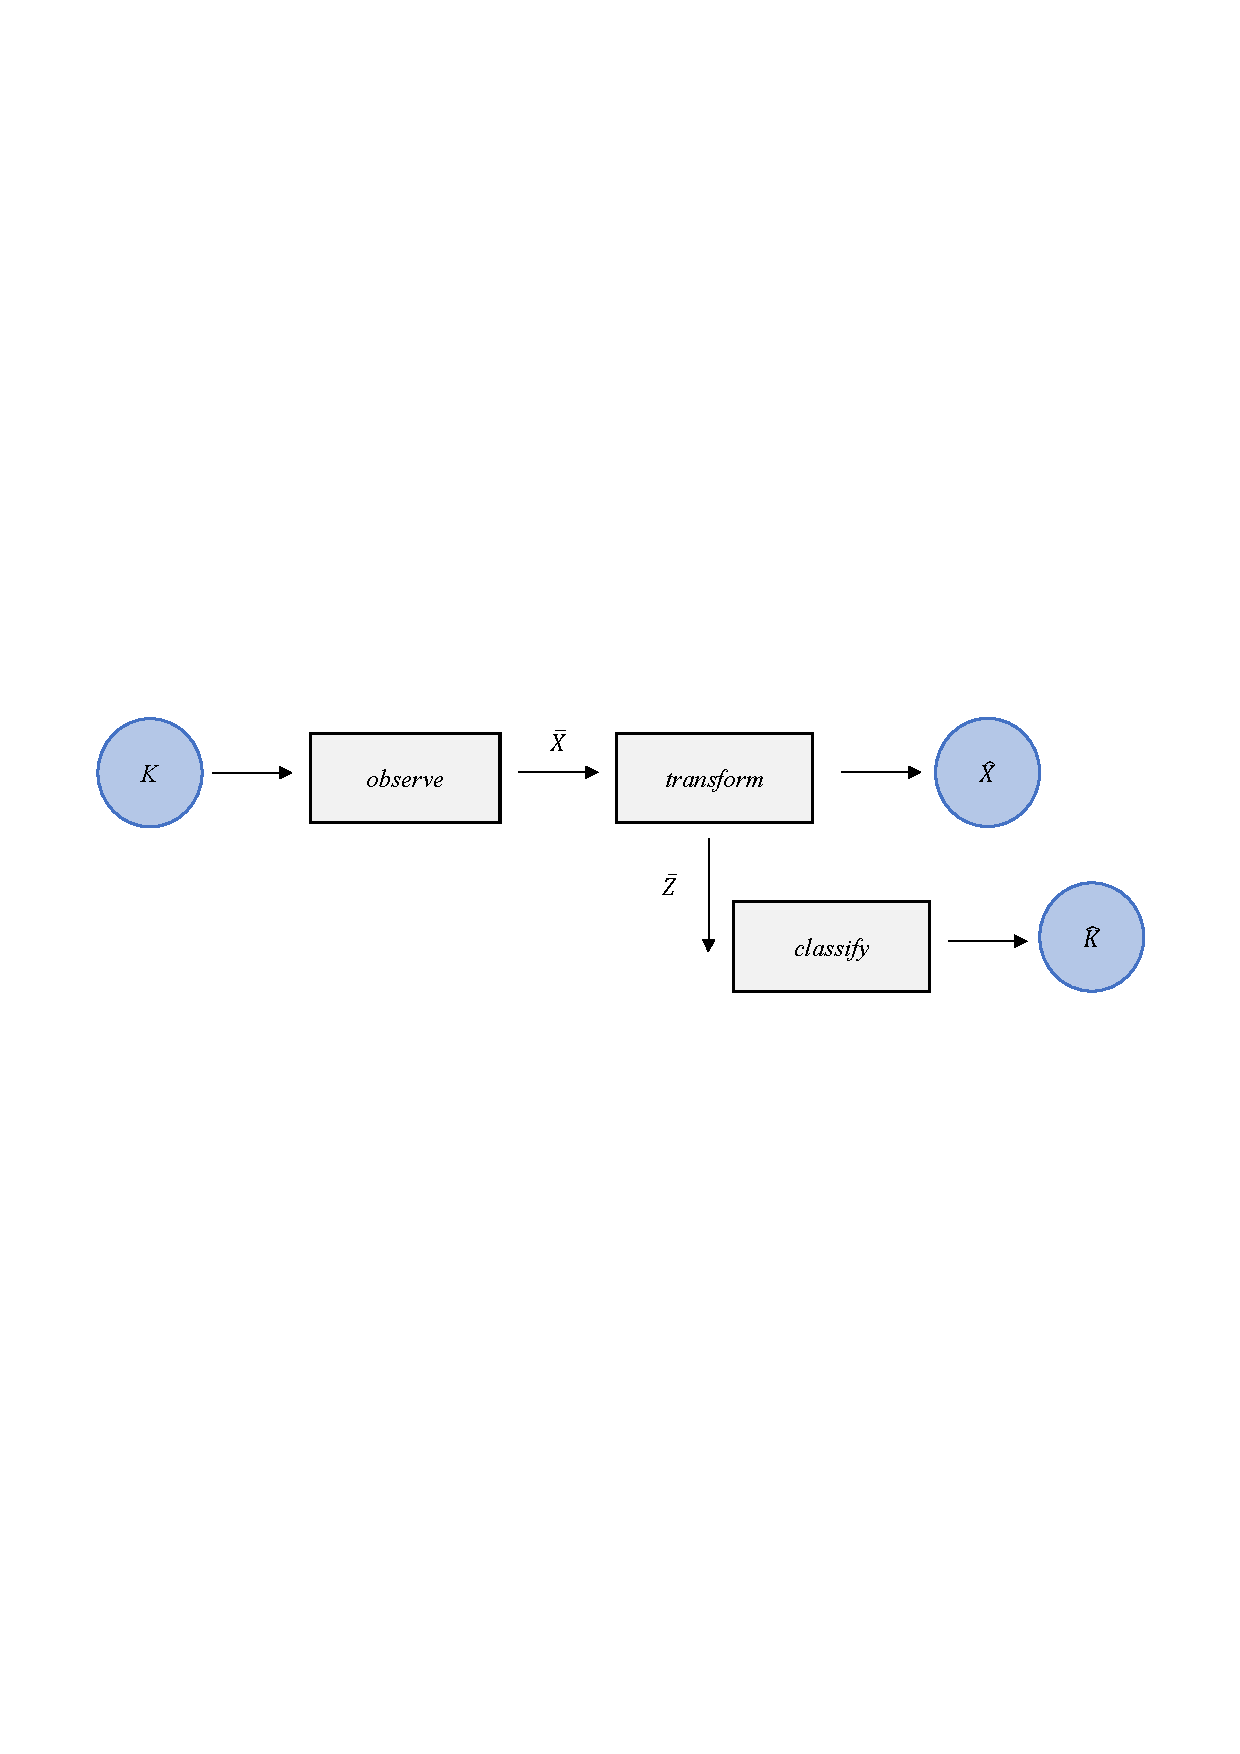
\includegraphics[width=16.5cm]{Figuras_tfg/Figura1_1_tfg}
		\caption{Our end-to-end scheme uses the information regarded from inside the transformation block and we then produce two outputs. First, the predicted $\hat{X}$ which we can use to measure our transformation accuracy. Secondly, $\overline{Z}$, which contains compressed information about $\overline{Z}$}
		\label{fig:fig1a} 
	\end{subfigure}%  
	\caption{Comparison between the classical view of a supervised classification in (a) versus the the model implemented for the purpose of this work in (b).}
	\label{fig:fig1}
\end{figure}

\section{Objective}

The model that I will be implementing will be an adaptation of the scheme on Figure~\ref{fig:fig1}.\subref{fig:fig1a}. To further investigate on the boundaries of Information transmission , I am using an \textbf{Autoencoder} to test the Information Bottleneck Principle~\cite{Inf_Bottleneck_first}.

In this report, I designed the following model which provides reliable information about the process of data compression and the limits of quantifiable information:
+
\begin{itemize}
	\item  We have a random source $K$ generating observations. Through a process of measurements, our system then will be provided with vectors of random observations $\overline{X}$. 
	
	\item The output observations  are then fed to the Autoencoder, which will then reduce the $\overline X$ into another vector $\overline Z$ with a different length but retaining the information from the input vector in a compressed from. 
	
	\item The Autoencoder also provides an output, which should be a reconstruction of the observations used to feed the Deep Learning structure. 
	
	\item The $\overline Z$ is then used for the classifying task of choice to output the predicted labels using a classifier of our choice. 
	
\end{itemize}

Note that Figure~\ref{fig:fig1a} follows a similar model to that of Figure \ref{fig:fig1}, but its transformation block is used to access the inside content of it rather than to provide a typical representation of an end-to-end transformation scheme. Although both of them typify a MIMO (Multiple Input Multiple Output) block, the Autoencoder is essentially an unsupervised transformation method, while the transformation block can be either composed by supervised or unsupervised task.\par


\section{Outline}

This report is divided into four Chapters, each one of them exploring different parts of the process of designing and testing the architecture proposed on Figure \ref{fig:fig1}:

\begin{itemize}
	\item \textbf{ \autoref{chap:Introduction}, Introduction} : Explains briefly the key concepts of the report as well as the cost of the project and the socio-economic impact of Big Data.
	
	\item \textbf{ \autoref{chap:TheoreticalBackground}, Theoretical Background} : Includes basic information about the theory and methods used in the Bachelor Thesis as well as the state of the art.
	
	\item \textbf{ \autoref{chap:ExpRes}, Experimental Results} : Presents key aspects to be aware of before starting the experimental phase of the project as well as the processes to obtain the results and the discussion associated with them.
	
	\item \textbf{ \autoref{chap:Conclusion}, Conclusion} : Final review of the project and the implications of it.
	
\end{itemize}

\section{Socio-economic environment}
\subsection{Budget}

The Budget for the project has been assigned according to three main costs : licenses, equipment and labour. The licenses used in this project are both included for Windows 10 and Mac OS X Mojave. On the other hand, the equipment includes the hardware and the resources needed for its adequate use. Finally, the labour costs are calculated using the metrics available at Indeed.com \cite{ProgrammerSalaries}, and then considering that each programmer works 8 hours daily, 22 days monthly and 12 months yearly. We are also going include a period of 300 working hours as the billing time for the Bachelor's Thesis \par
\begin{table}[H]
	\caption{Total budget costs table}
	\label{tbl:budget_table}
	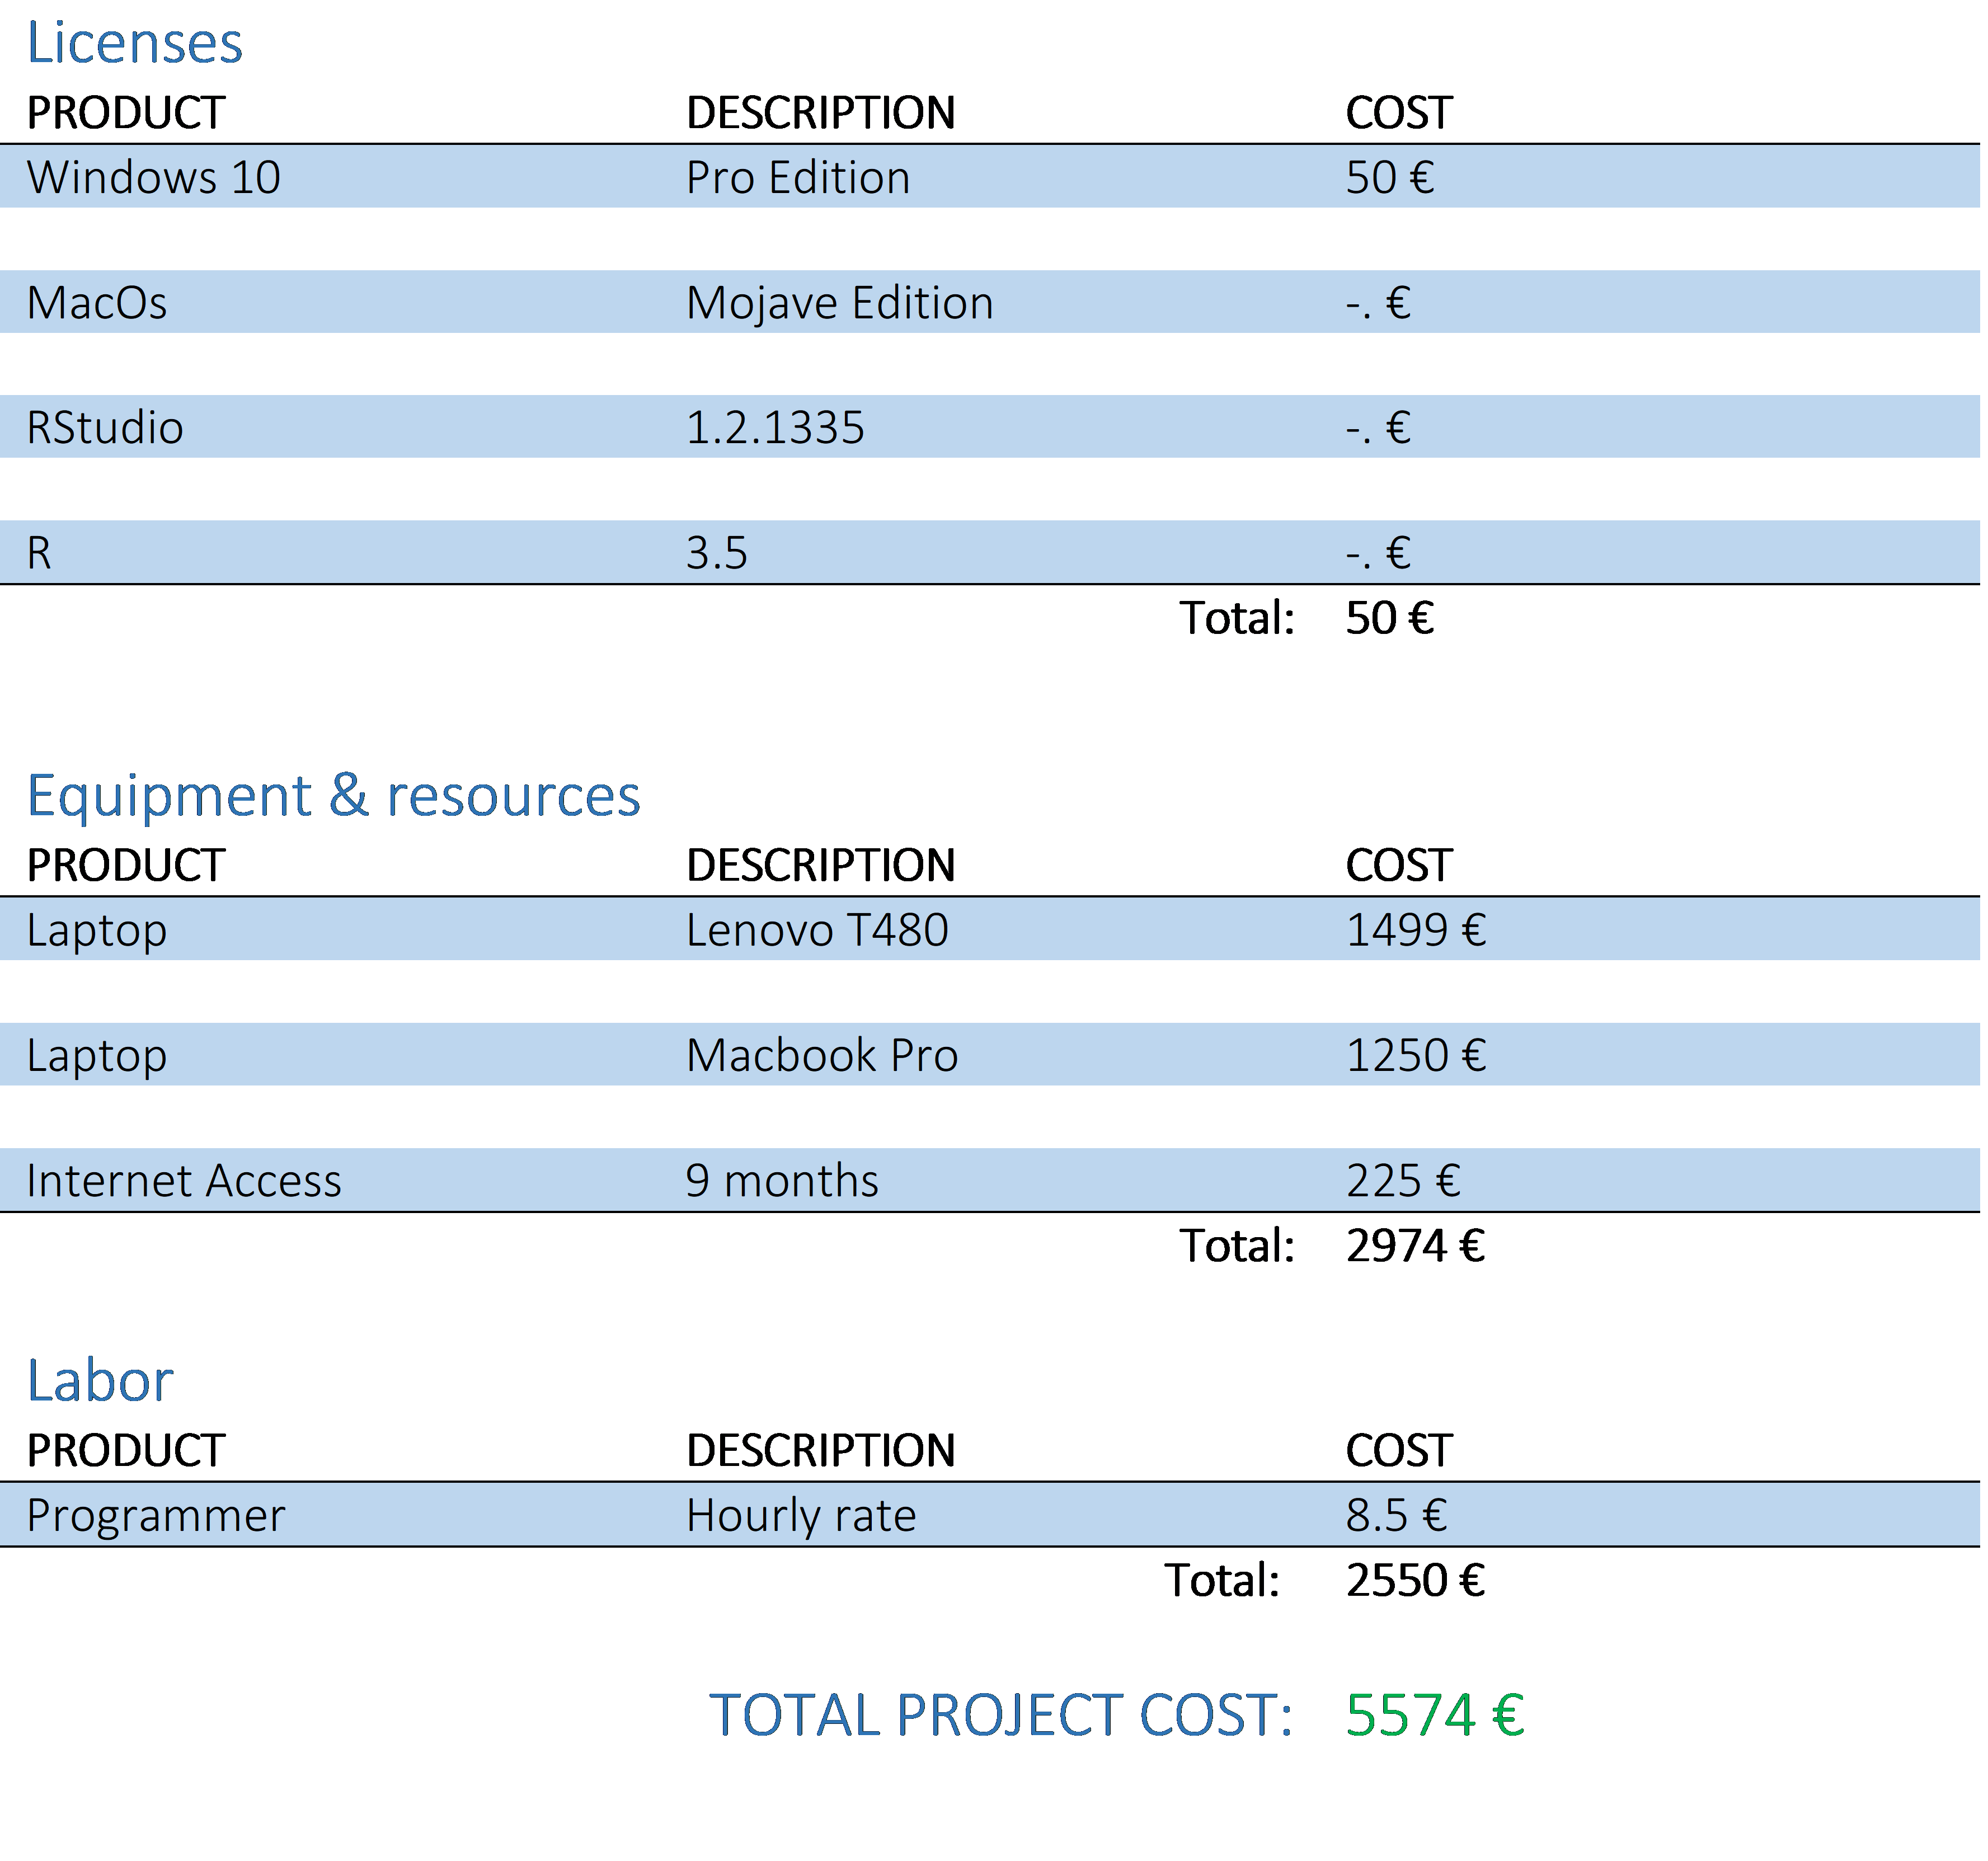
\includegraphics[width=\linewidth]{Table_Costs.png}
\end{table}

\subsection{Socio-economic relevance}

Big Data and Neural Networks have been referred as two of the major innovations of our decade. Many mainstream media articles have appeared in recent years discussing the impact that it will have in our lives~\cite{Forbes_Article}. Economic agents have been working on their development and how it will affect the way business are conducted in our modern era. In the same way, people have started to realize that data analytics and the management of information are important topics that affects each and everyone of us.

In this context, assessing the validity of results and their reliability becomes a must. From the medical field, where data can be critical to find the cure for a specific disease~\cite{Nature_Article}, to designing safety systems and creating better customer relationships for aviation companies~\cite{Article_Aviation}, it is highly important for researchers to improve their methods to solve Big Data problems so they are able to find the correct solutions to these challenges. Moreover, thanks to the advances in hardware and information available to the public, everyone has access to a wide variety of information on the topic of Big Data. Taking all these points into account, establishing an empirical tool that is able to polish research and strengthen results in the data analytics field can have a positive impact that affects all stakeholders.

To sum up, Big Data has changed the way society is and by improving it we can be able to shape the technology and lives of tomorrow's people.

\section{Regulatory framework}

The regulatory framework of this project can be closely related with Regulation 2019/679 of the European Parliament, also known as General Data Protection Regulation~\cite{GDPR}. The aim of this law is to protect the privacy of all of the individual citizens of the European Union (EU) and the European Economic Area. The GDPR gives the people of the EU the control of their personal data, which protects them from violations related to the use of their personal data in processes like Big Data or Data Analytics without their consent. It is also divided into eleven chapters, each one of them referring to different aspects of the legislation. 

If data was to be used replicating the procedures presented in the Bachelor Thesis for commercial use (thus not applying Recital 18), some pieces of the regulation must be specially taken into consideration before doing so. %\newline

\begin{figure}[H]
	\caption{View from the outside of the European Parliament.}
	\label{fig:European_Parliament}
	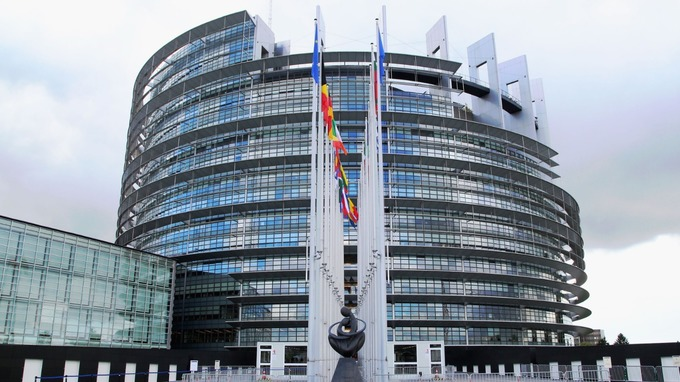
\includegraphics[width=\linewidth]{European_Parliament}
\end{figure}

Although all of the chapters introduced in the document are related to the topic of Big Data, as the possible holders of data we must take a deeper look into Chapter~\ref{chap:ExpRes}, which accounts for the rules that are to be applied to the data controller. 
%
A list  of Articles that apply---and in which respect---follows:
%
\begin{itemize}
	\item \textbf{Article 25} requires private data to be stored using the appropriate measures, and by further reading into it we see that Recital 78 mandates to store the data in such a way that it cannot be traced back to the source without additional information.To protect our user's from having their private information stolen and used against them, a proper way to store their data would be to don't use direct references to qualities or traits from the individuals included in the datasets, and to rather use other representations of it. For example, if we used transformed observations by applying BoxCox or any other type of pre-processing with certain unknown parameter only available for us before saving it, we could avoid risking our users personal information while still keeping the purity of our information. An example of that transformation is included in \autoref{chap:ExpRes}.
	
	\item At the same time, \textbf{Article 30} states that the processing activities related with such personal information must be recorded and kept. We comply with this directive due to the fact that the development of this Bachelor's Thesis has been recorded by regular uploads to a public repository in Github.
	
	\item  If a security break happened and private information from the users is compromised, \textbf{Article 33} mandates that the supervisory authority must be notified unless the breach is unlikely to affect individual rights. As the proprietor for this project, this role would be assigned to me in case of it happening.
	
	\item In case that the accessed information is likely to risk the rights and freedoms of a person, the individual must be notified (\textbf{Article 34}). Again, as the proprietor of the work, this would be performed by me. 
	
	\item To avoid breaches and help secure individuals' data,\textbf{Article 35} accounts for data protection impact assessments to be conducted if specific risks arise. No risks were assessed as no personal data was used during the experiments.
	
	\item \textbf{Article 37} requires a data protection officer to be designated in order to assist in the monitoring of the compliance with the Regulation and, in case of criminal conduct, measures have to taken by the regulatory agency (\textbf{Article 9} and \textbf{Article 10}). This article applies to me as my role of the proprietor of the Bachelor's Thesis.
	
	\item  Organizations outside of the EU must also appoint a representative (\textbf{Article 27}). No representative would need to be appointed as this Bachelor's Thesis was based in Spain, inside of the EU.
	
\end{itemize}  

This Bachelor's Thesis complies with all of the Articles from the GDPR since no personal data was acquired or used for the purpose of our experiments. In case of performing the methods mentioned with the purpose of gaining financial benefit by using personal data, the previous guidelines should be followed to secure the privacy of the individual's information involved in the experiments. \par




